A experiential method based on measurements is used to make the PL model, that will be used to calculate the loss for near ground communication. This model is based on data gathered from measuring the PL at different heights and distances. In each point there will be taken multiple measurements, so the noise factor will have a less of an effect on the results.

During testing, five sets of antennas are used, a set monopole antennas (858 MHz) a set patch antennas (858 MHz). By using two different sets of antennas, it can be taken into account if the antenna type will have a influence on the results of the measurements. 

There will also be tested with horizontal and vertical polarization, to see if this will effect the model. The testing will take place at two locations, outside an empty parking lot and inside a gym (45 by 25 meters). Two locations is used, to see if the model works at two different locations.

%\begin{figure}[!htbp]
%\centering
%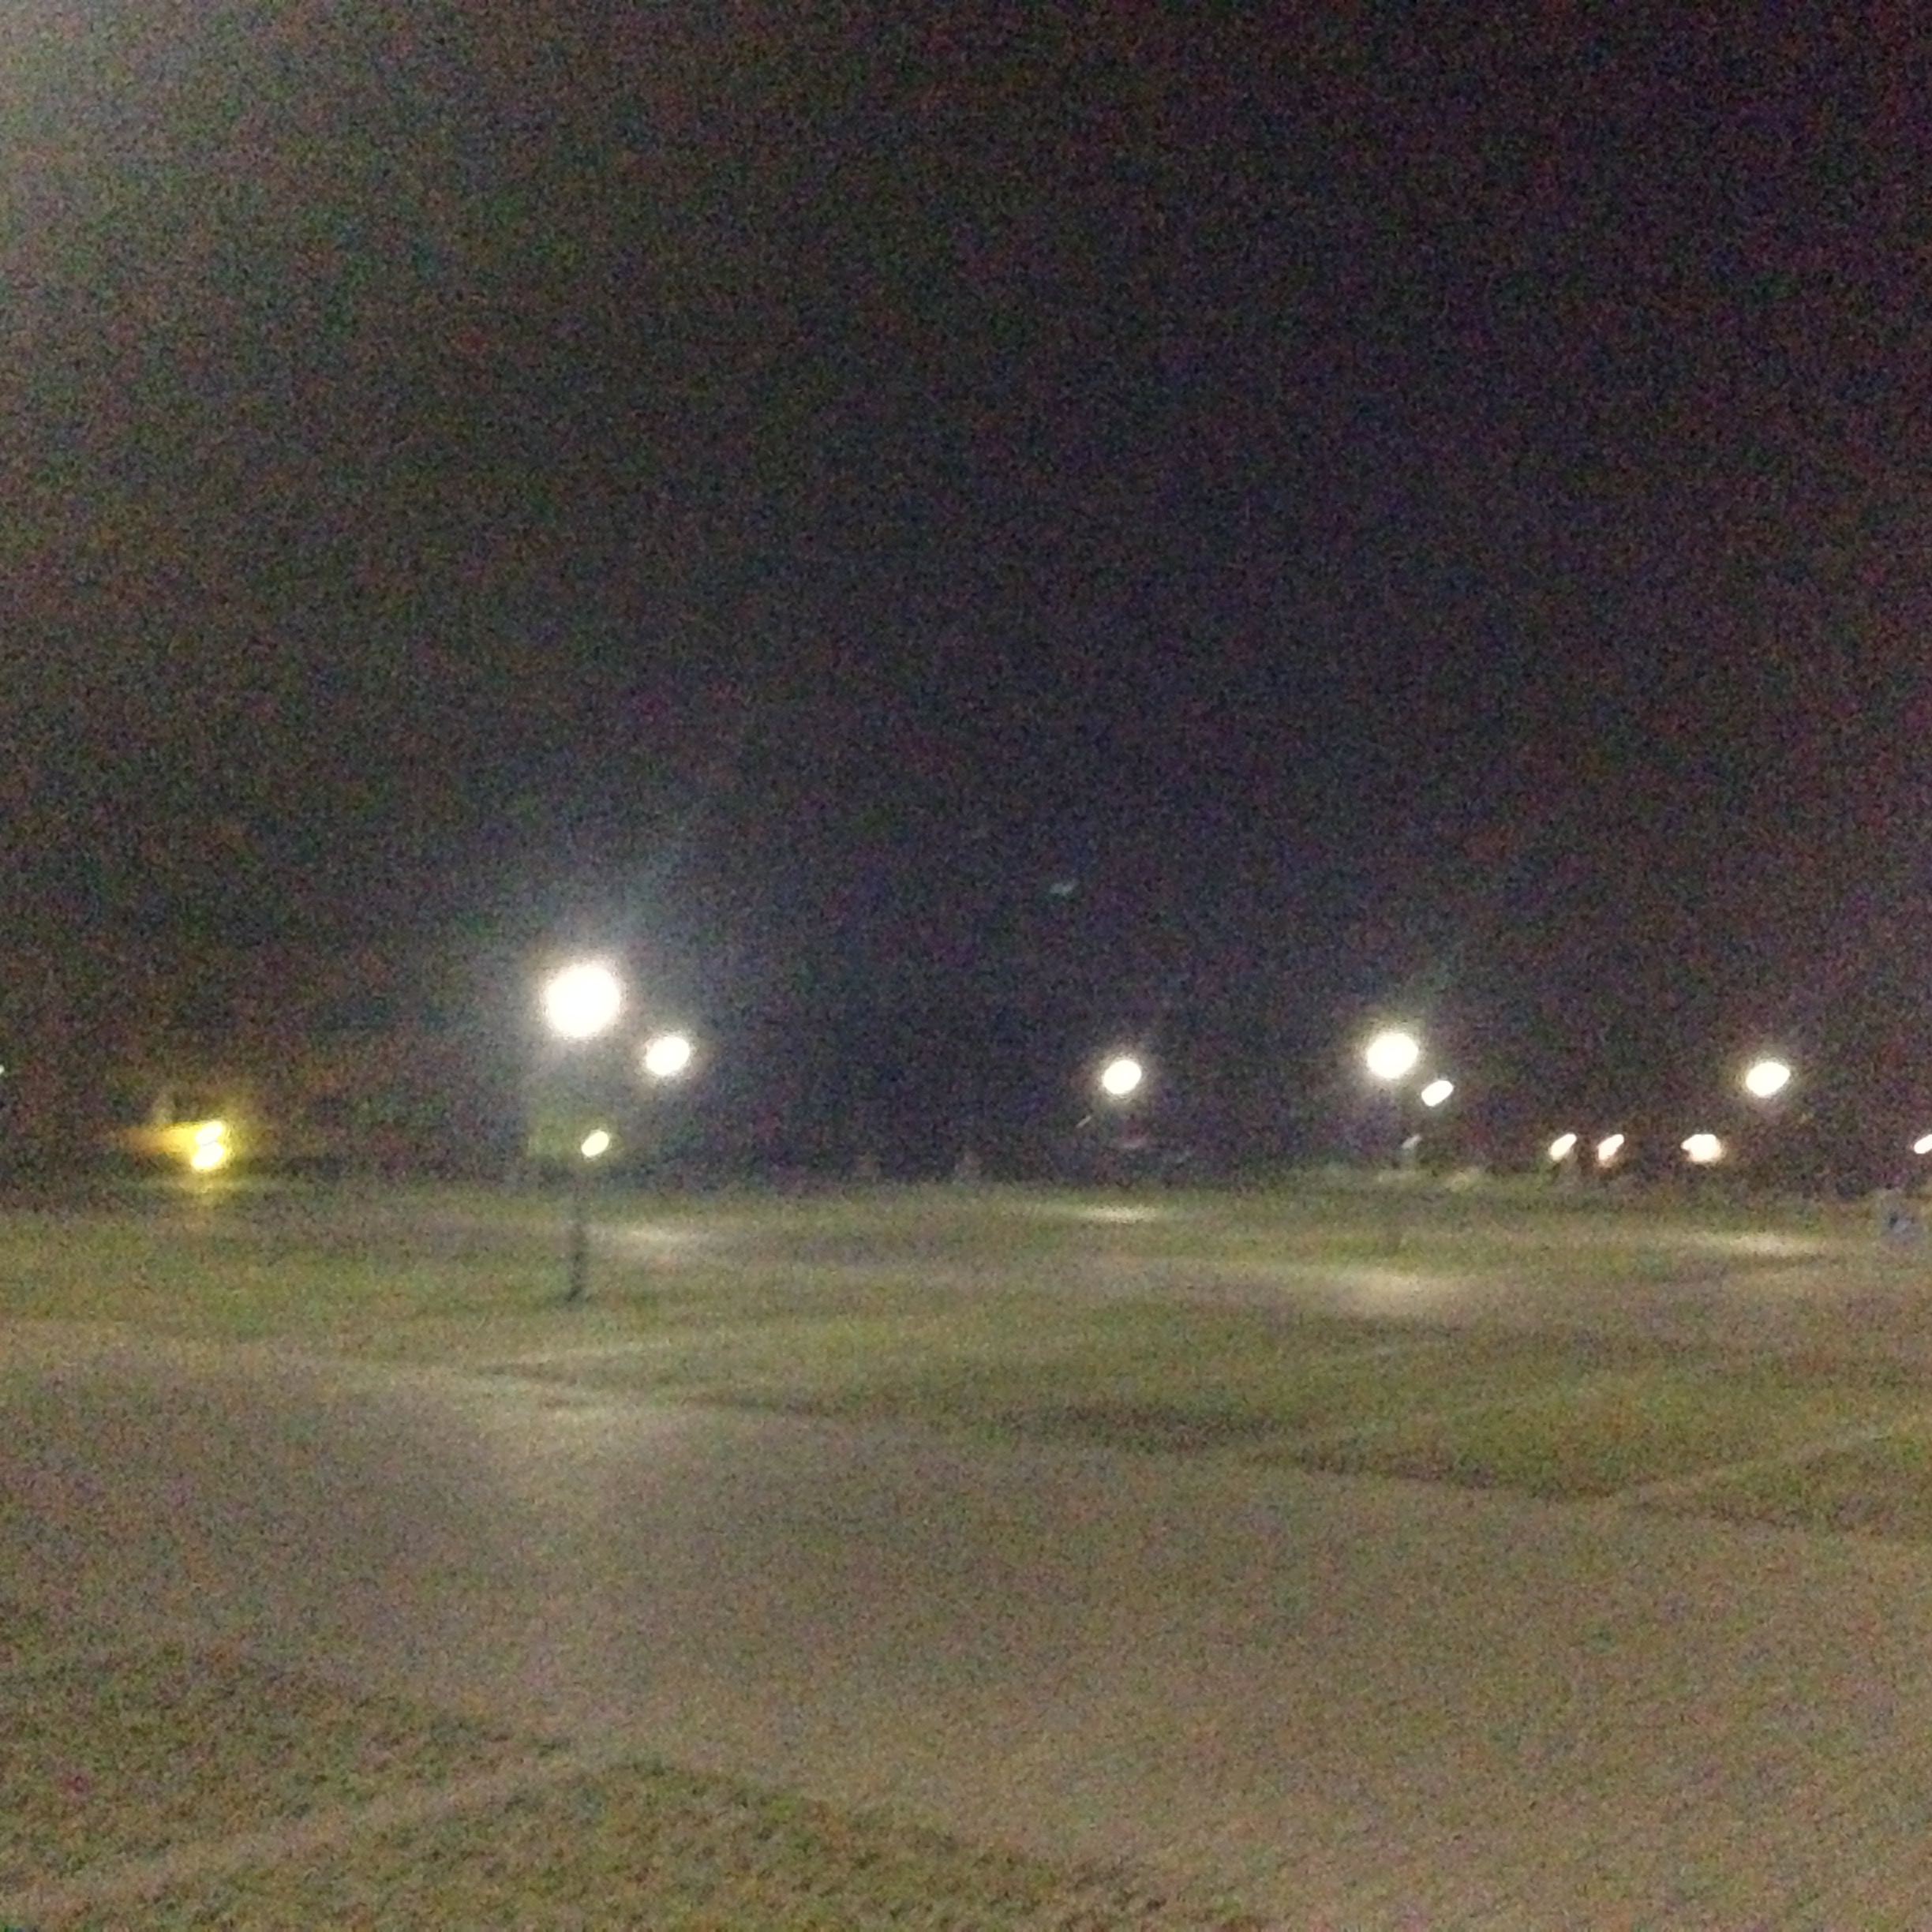
\includegraphics[width=0.2\textwidth]{Pplads.jpg}
%\caption{Illustration of the First and Second Fresnel zone, along with the Direct signal travelling from the Transmitter TX to the Receiver RX}
%\label{dijdk}
%\end{figure}


\begin{figure}
\centering
\begin{minipage}{.2\textwidth}
  \centering
  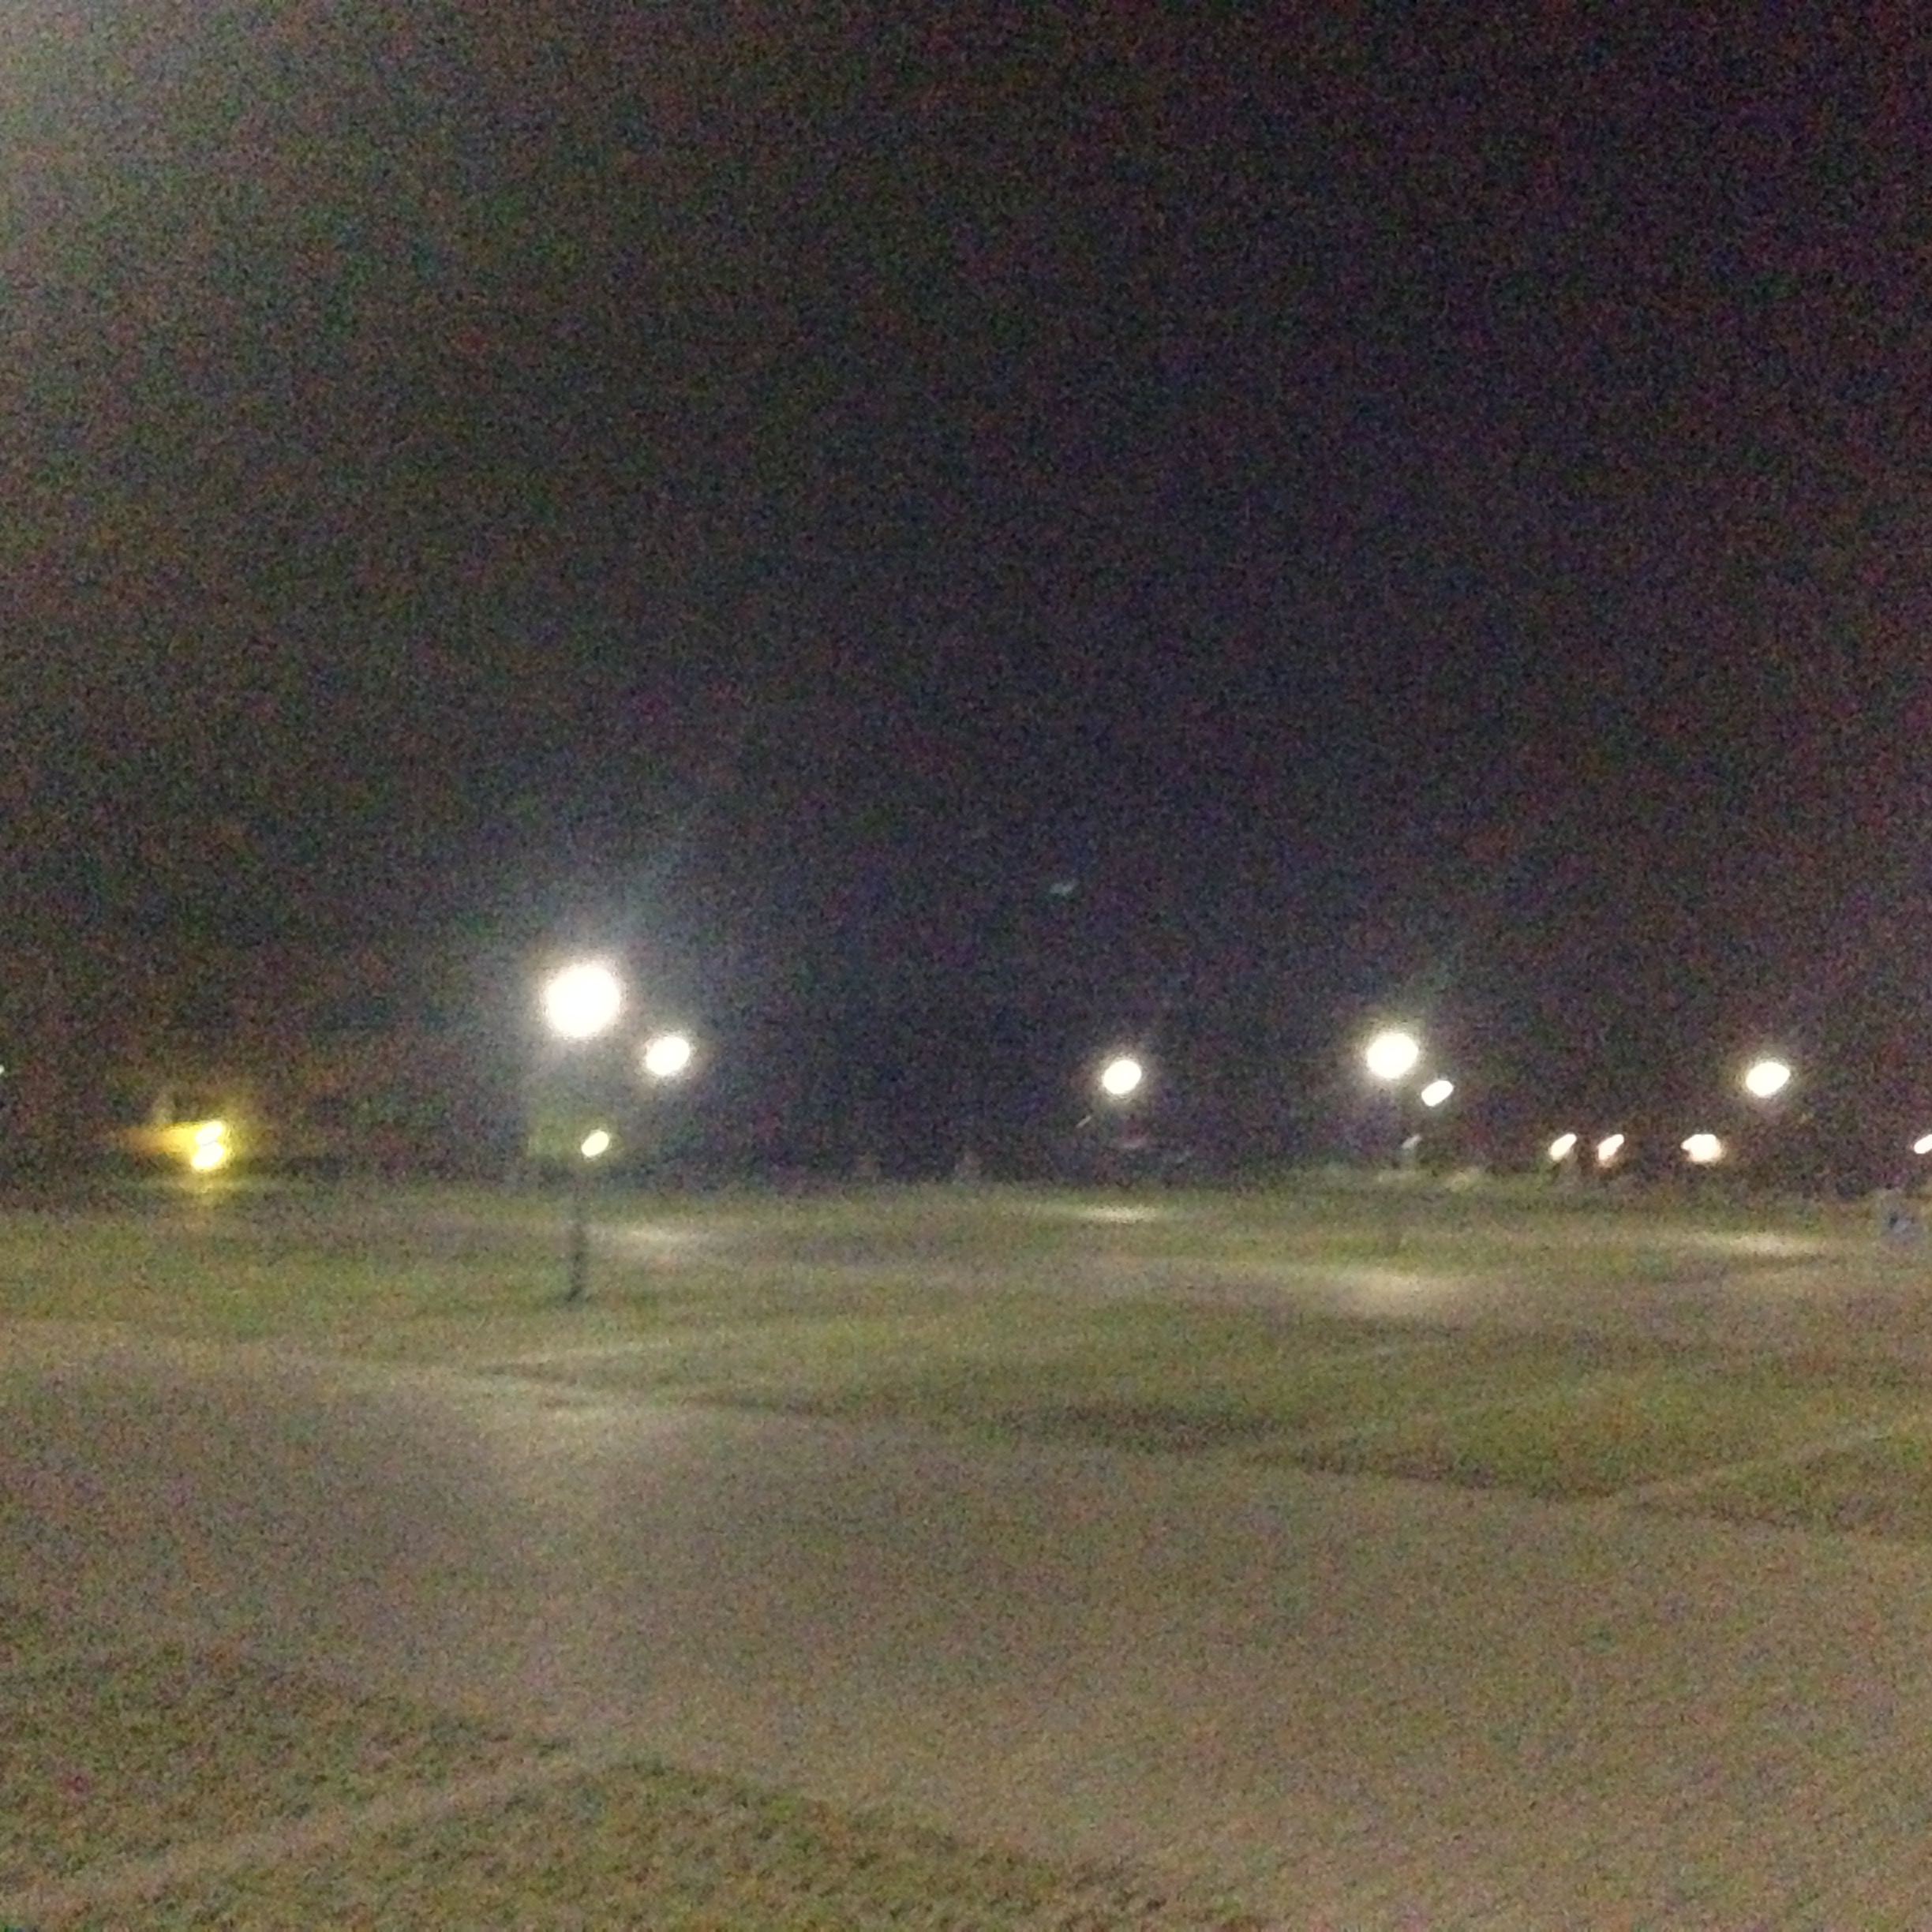
\includegraphics[width=\linewidth]{Pplads.jpg}
  \captionof{figure}{Measurement at the empty parking lot}
  \label{fig:test1}
\end{minipage}%
\hspace{2mm}
\begin{minipage}{.2\textwidth}
  \centering
  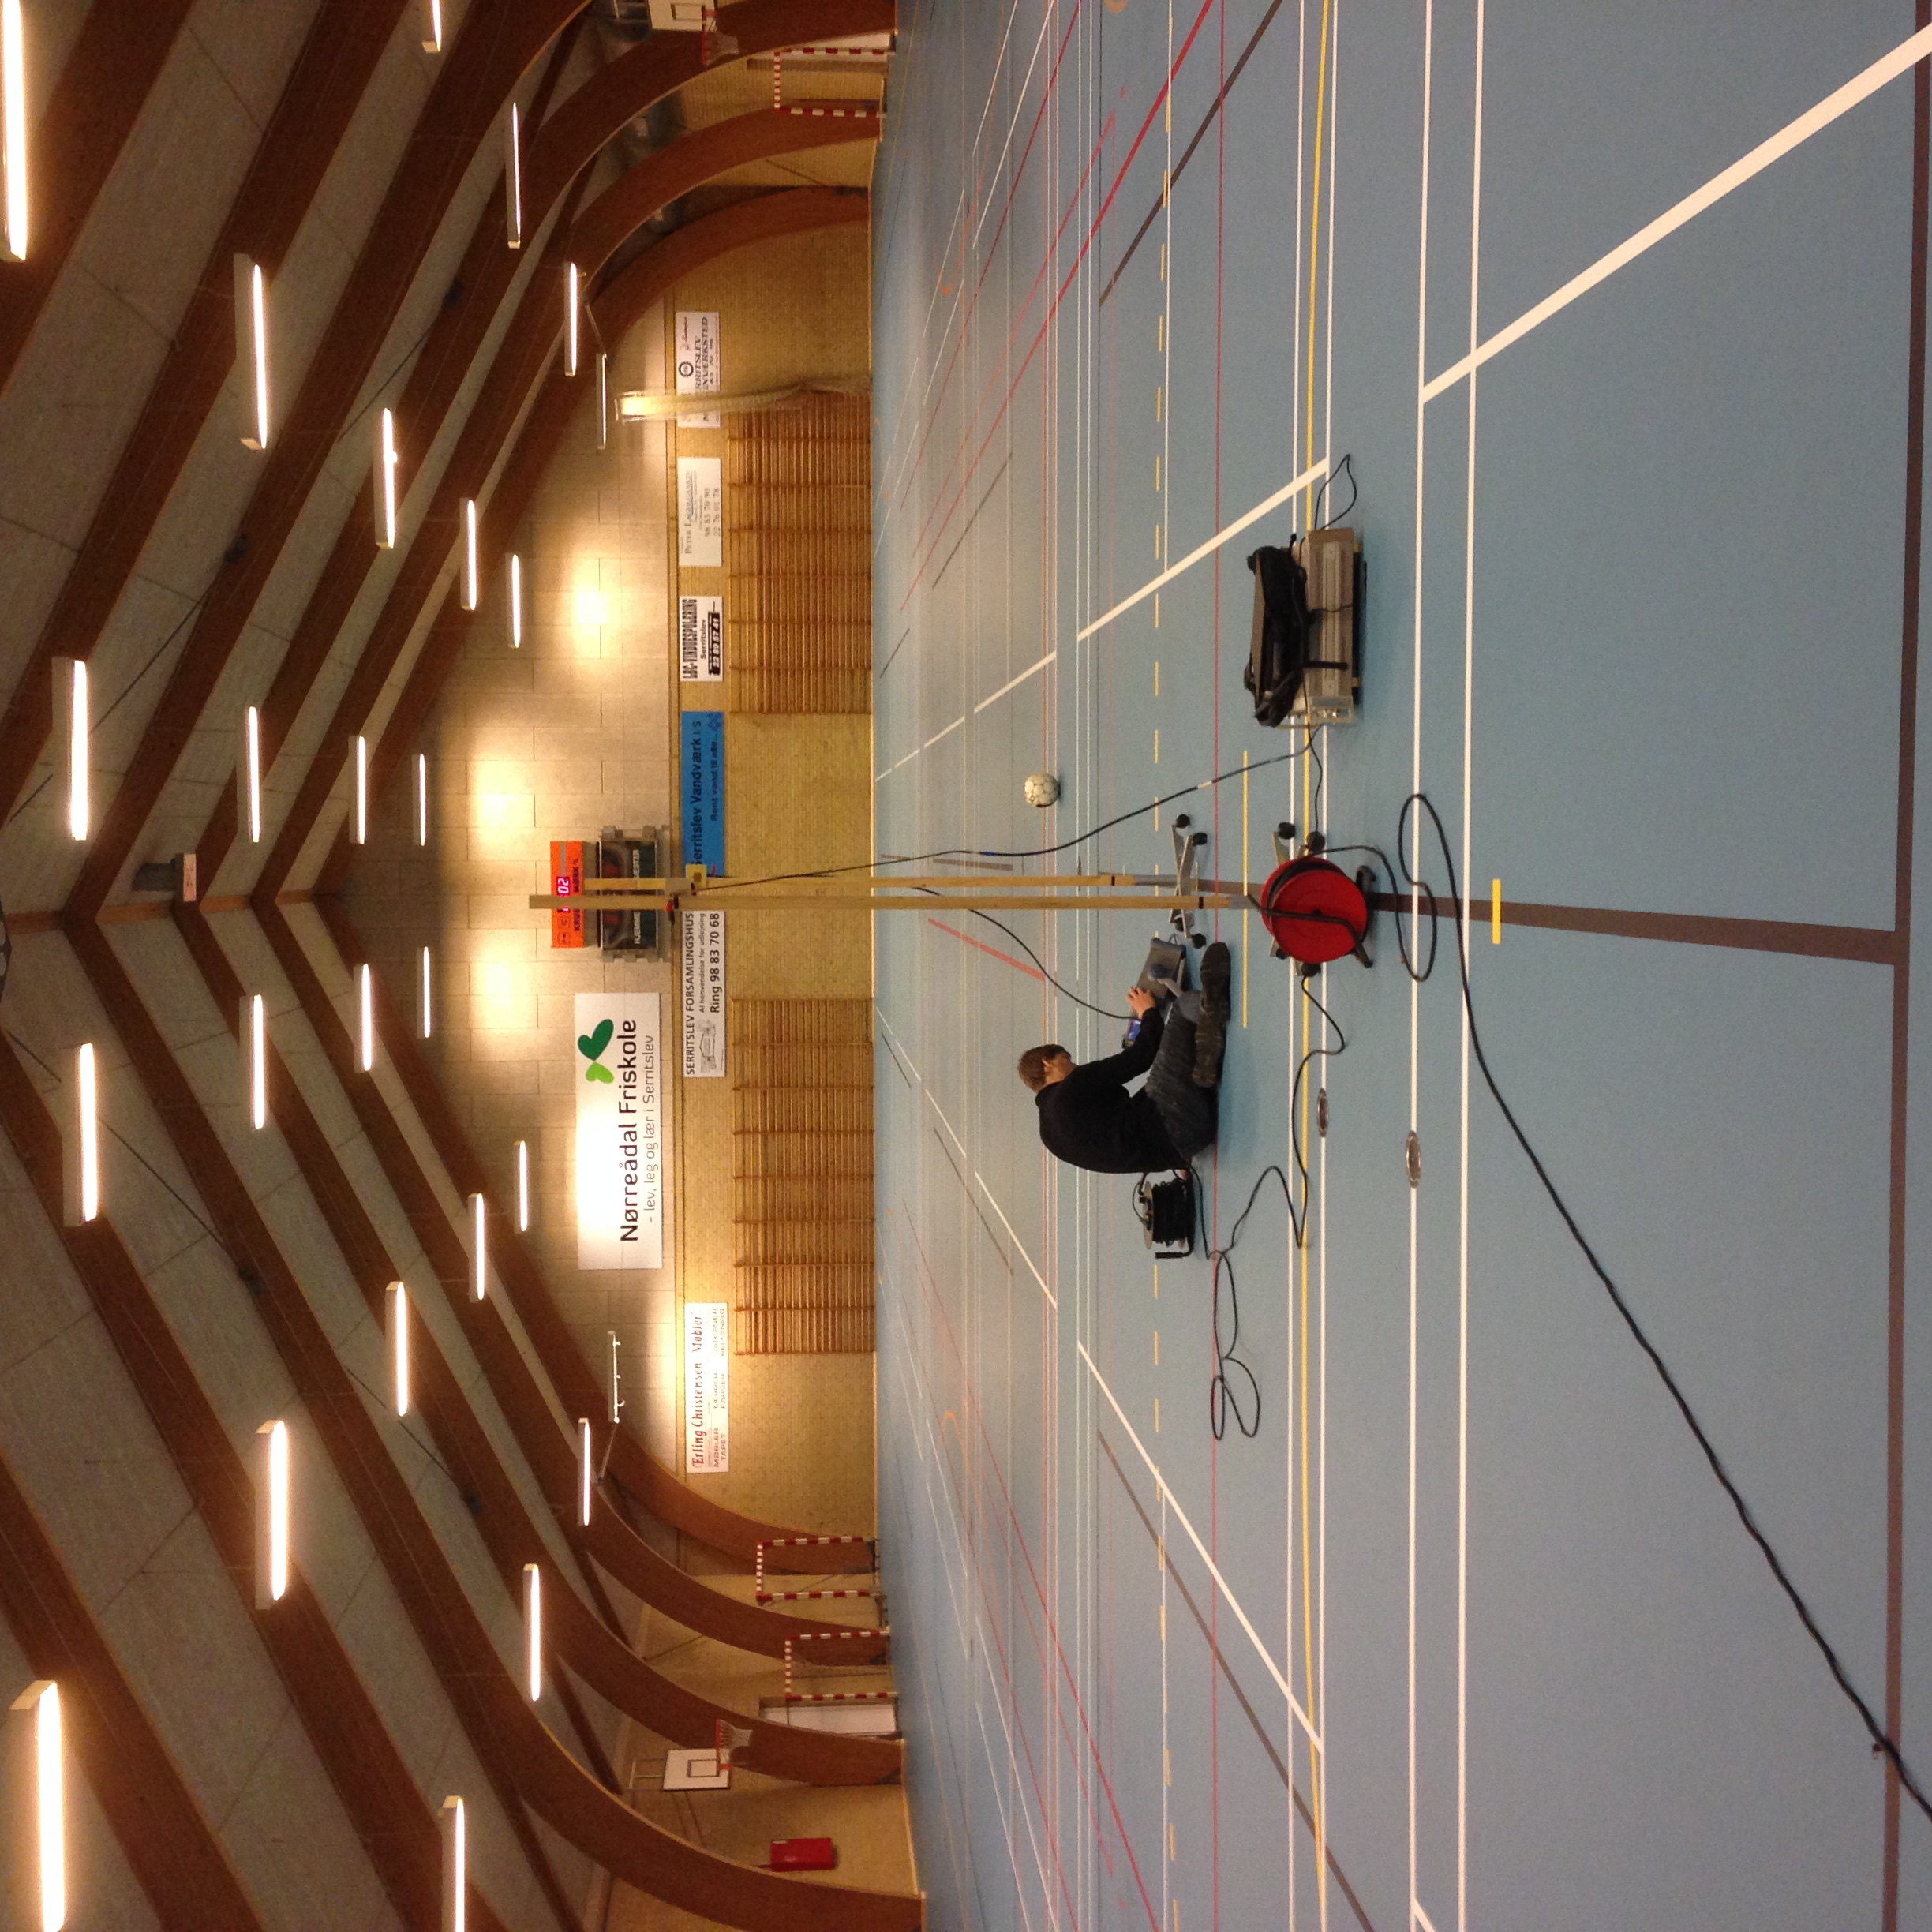
\includegraphics[angle=-90, width=\linewidth]{Hal.jpg}
  \captionof{figure}{Measurement at the gym}
  \label{fig:test2}
\end{minipage}
\end{figure}

